% !TEX root = ../thesis.tex


\chapter{Theoretical Background}
\label{cha:dmd_theory}
This chapter will cover the relevant theoretical background of digital mirror devices and the techniques used in conjunction with them. I will also give a short introduction for the experiment in our group that currently uses DMDs to generate optical box potentials. Finally, I will briefly cover some of the previous works that have been done on DMDs in our research group.

\section{Digital Micromirror Device}
\label{sec:digital_micromirror_device}
A digital micromirror device (DMD) is one form of spatial light modulator (SLM). It provides the user with the ability to imprint almost arbitrary patterns onto a beam of light and it can therefore be used to generate optical potentials for atom traps. A DMD is a rectangular array of square mirrors that form a pixel-like structure, very similar to how emanating displays are made of pixels. On the DMD screen however, the pixels work by tilting mirrors along their diagonal which gives each pixel two distinct positions (see Fig.~\ref{fig:dmd_example}). The direction of light which will be used is called the \emph{ON} position while the other is correspondingly called the \emph{OFF} position. \cite{texasinstruments:2018}
%
\begin{figure}[htbp]
    \centering
    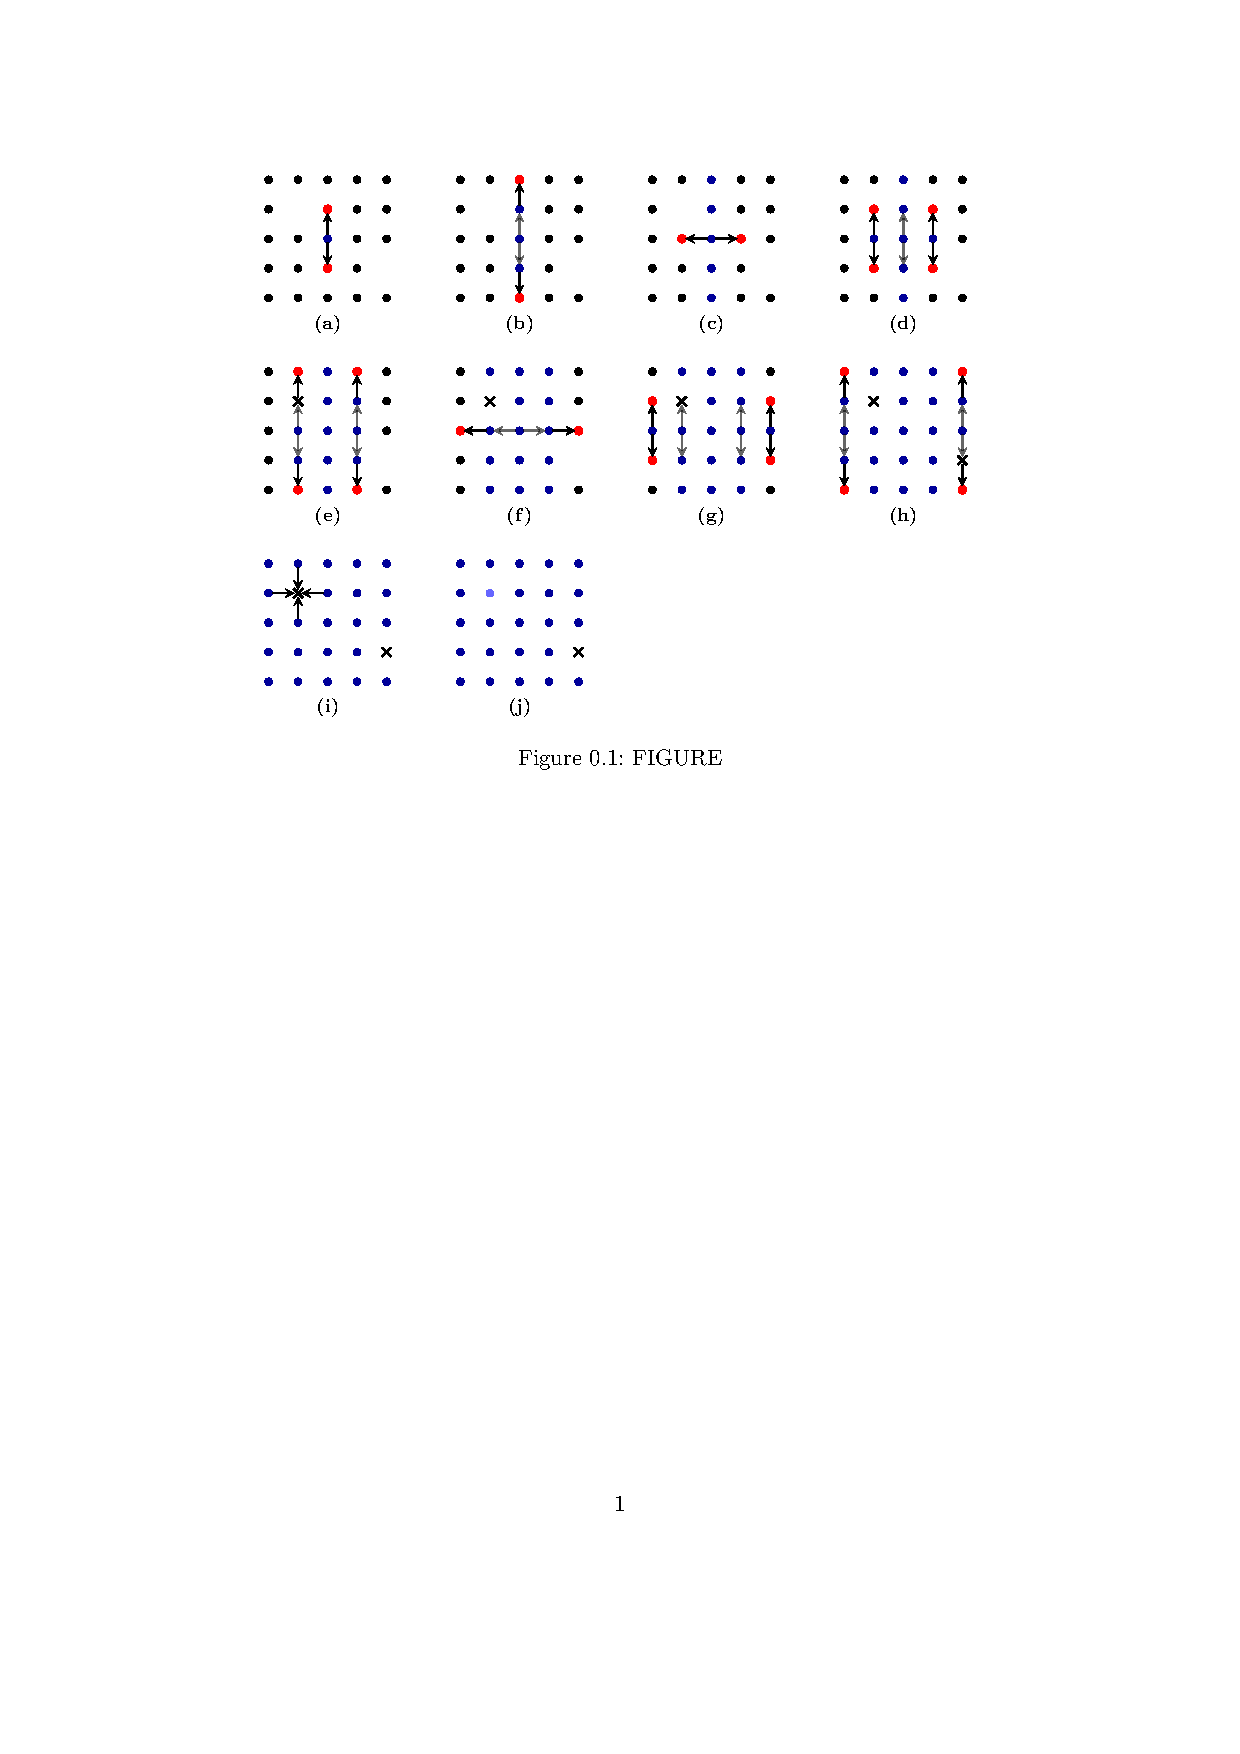
\includegraphics[]{DMD/Sketch/test}
    % \input{TexContents/Figures/DMD/Sketch/sketch.tikz}
    \caption[Close-up image of a chessboard pattern on a DMD]{Adapted from \cite{krstajic}. Close-Up image of a chessboard pattern on a DMD. The pixelated array of micromirros produces an image by tilting individual pixels by \SI{12}{\degree} along a diagonal hinge.}
    \label{fig:dmd_example}
\end{figure}

\noindent
From the discrete \emph{ON}/\emph{OFF} states it is obvious that DMDs can only produce binary patterns. In an experimental context however, it would be useful to produce grayscale images. For this, we can use the resolution properties of the optical system that images the beam from the DMD onto the desired plane. If the minimum resolvable structure is bigger than a single pixel, the intensity is averaged. For example, if a $3\times 3$ area of pixels is resolved as one spot, there are 10 shades available. However, we still deal with images on a pixel by pixel basis on the DMD and therefore need to convert a grayscale image into binary such that the averaged intensity remains as close to the original as possible.

\subsection*{Dithering}
When the colour depth of an image, i.e.\ the total number of shades available for displaying it, is reduced, quantisation errors occur \cite{funkhouser:2000}. For example, if we were to diplay a grayscale image with constant \SI{75}{\percent} brightness using only black and white, we could simply use rounding as the quantisation method. However, in this case it would result in a completelely white picture as each pixel is brighter than \SI{50}{\percent}. Instead, it would be better to use white pixels for \SI{75}{\percent} of the image and black pixels for the remaining \SI{25}{\percent} as this would again result in an average brightness of \SI{75}{\percent}. This process of artificially introducing noise to reduce quantisation errors is called dithering and is demonstrated in Figure~\ref{fig:dmd_dithering_example}. 
\begin{figure}[htbp]
    \centering
    \begin{subfigure}[t]{0.24\linewidth}
        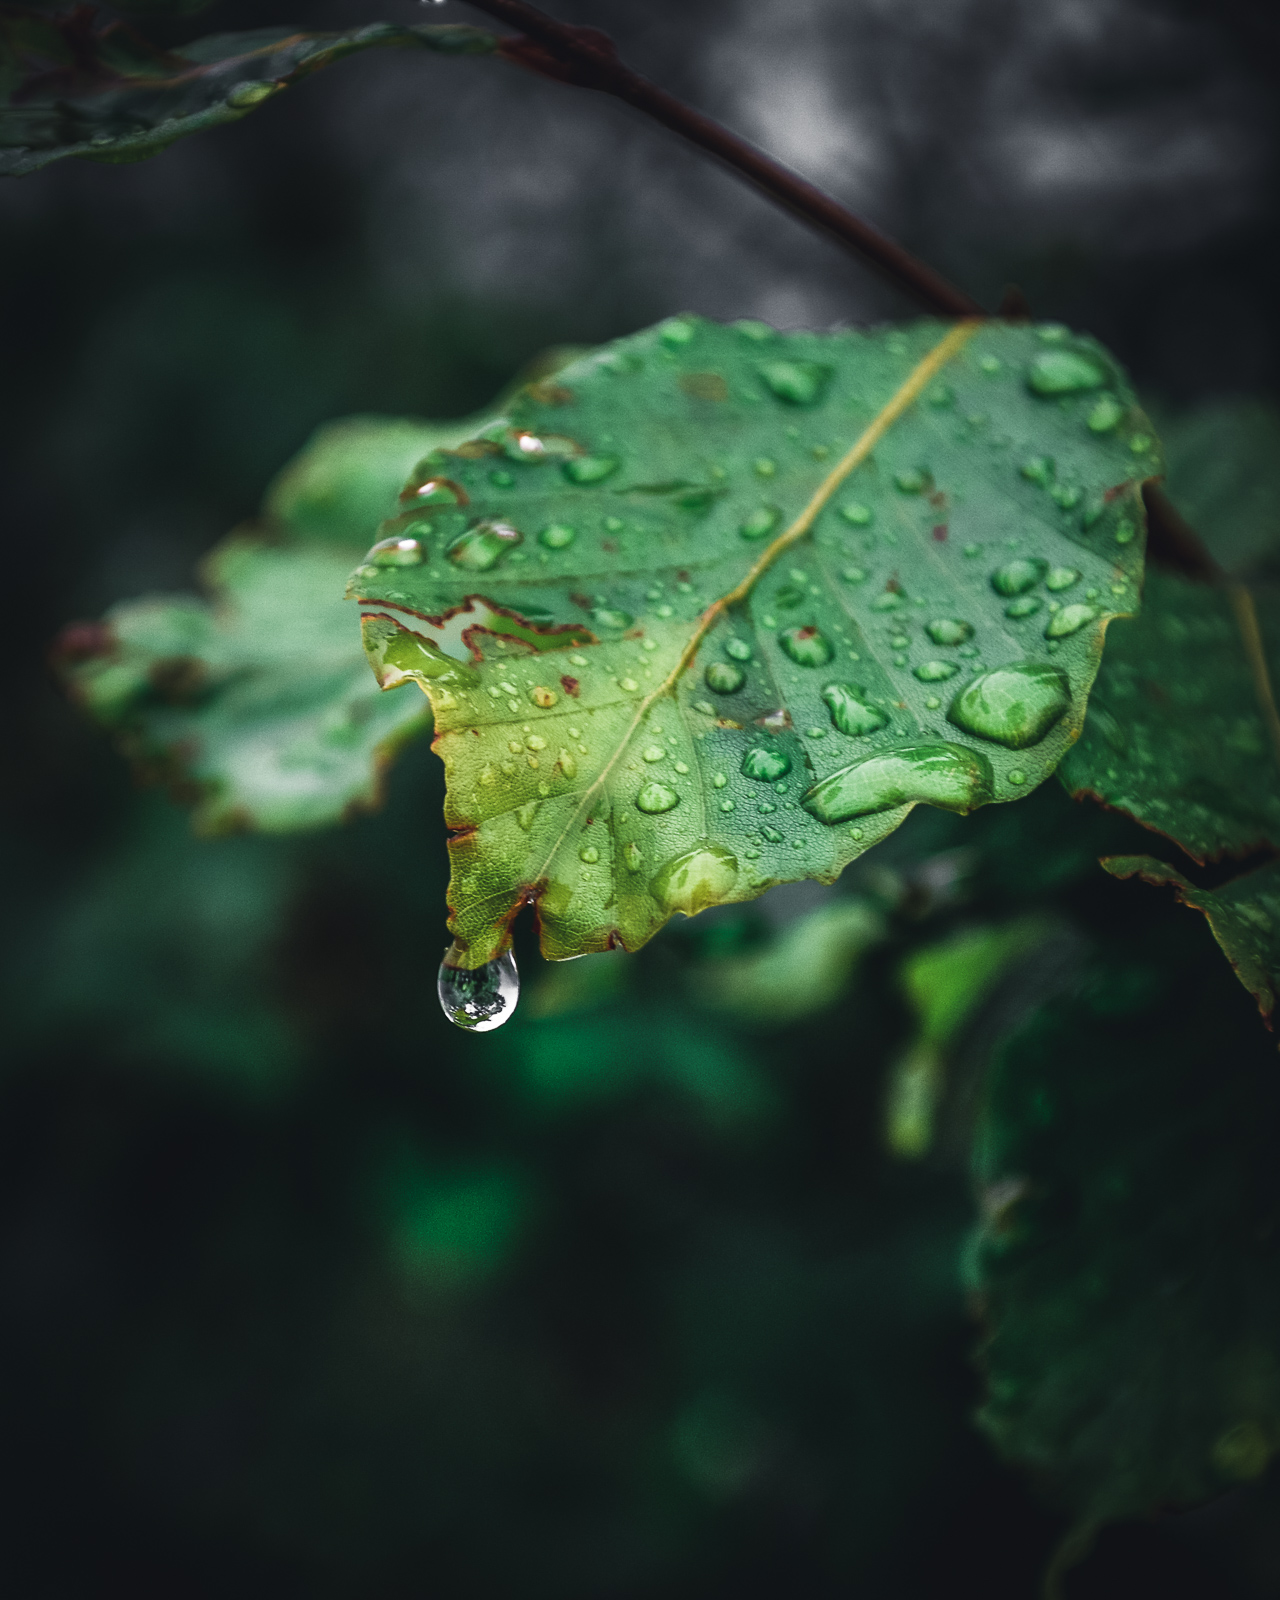
\includegraphics[width=\textwidth]{DMD/DitheringExamples/leafFullColour}
        \caption{\SI{24}{bit}, \num{16.8e6} colours}
    \end{subfigure}
    \begin{subfigure}[t]{0.24\linewidth}
        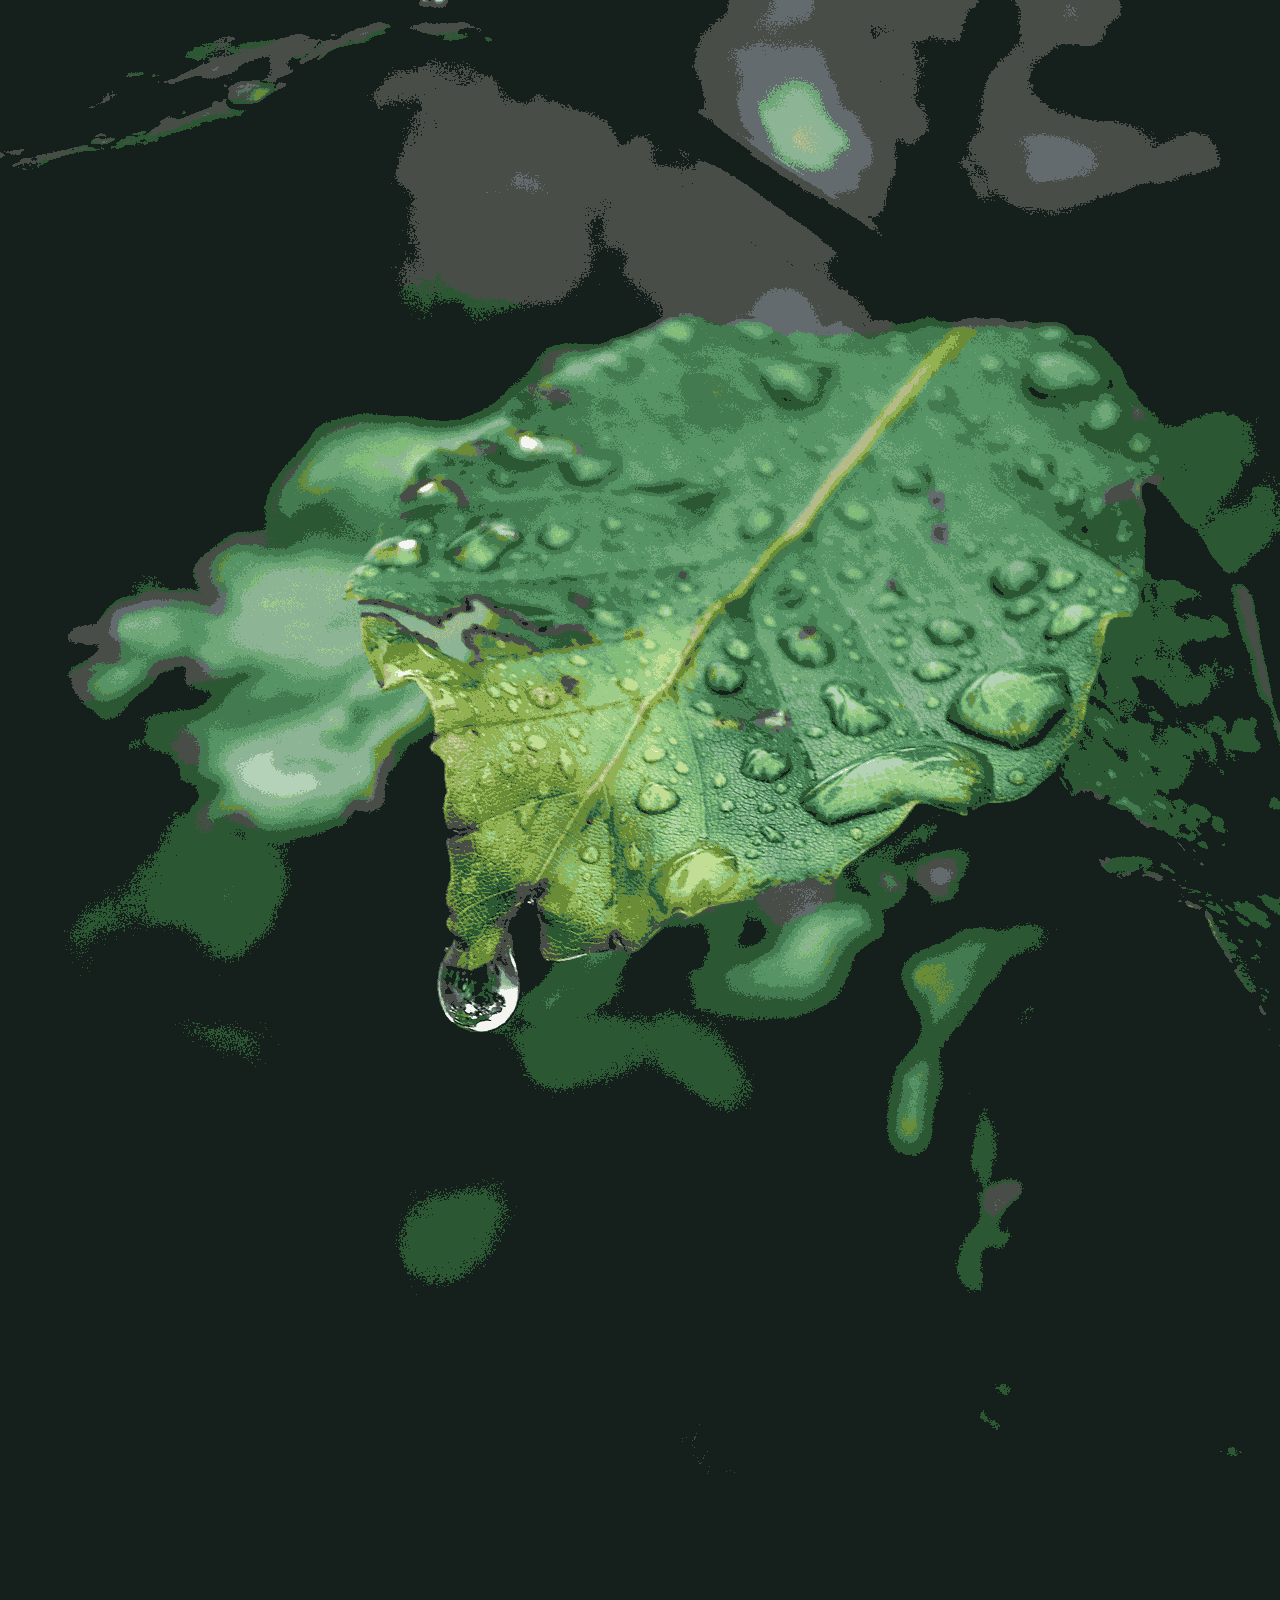
\includegraphics[width=\textwidth]{DMD/DitheringExamples/leaf16nodither}
        \caption{16 colours, without dithering}
    \end{subfigure}
    \begin{subfigure}[t]{0.24\linewidth}
        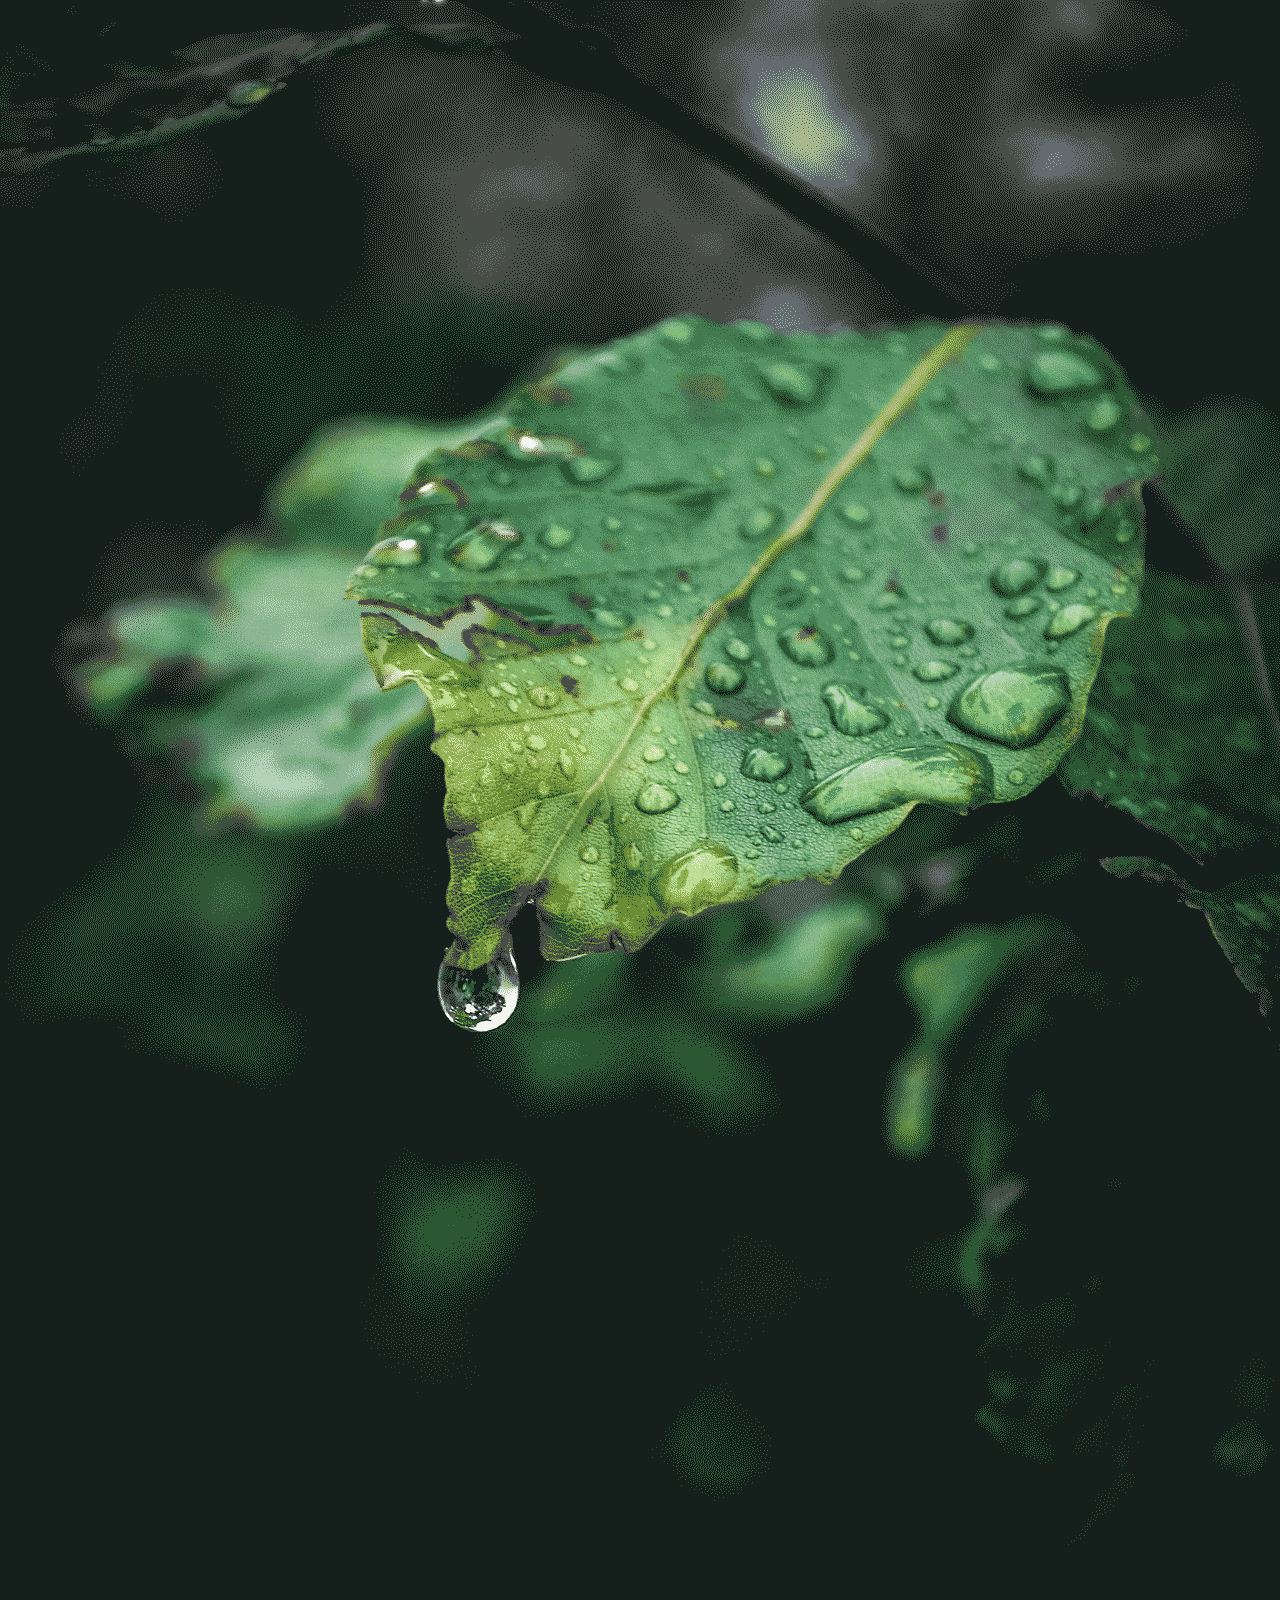
\includegraphics[width=\textwidth]{DMD/DitheringExamples/leaf16dither}
        \caption{16 colours, error diffusion}
    \end{subfigure}
    \begin{subfigure}[t]{0.24\linewidth}
        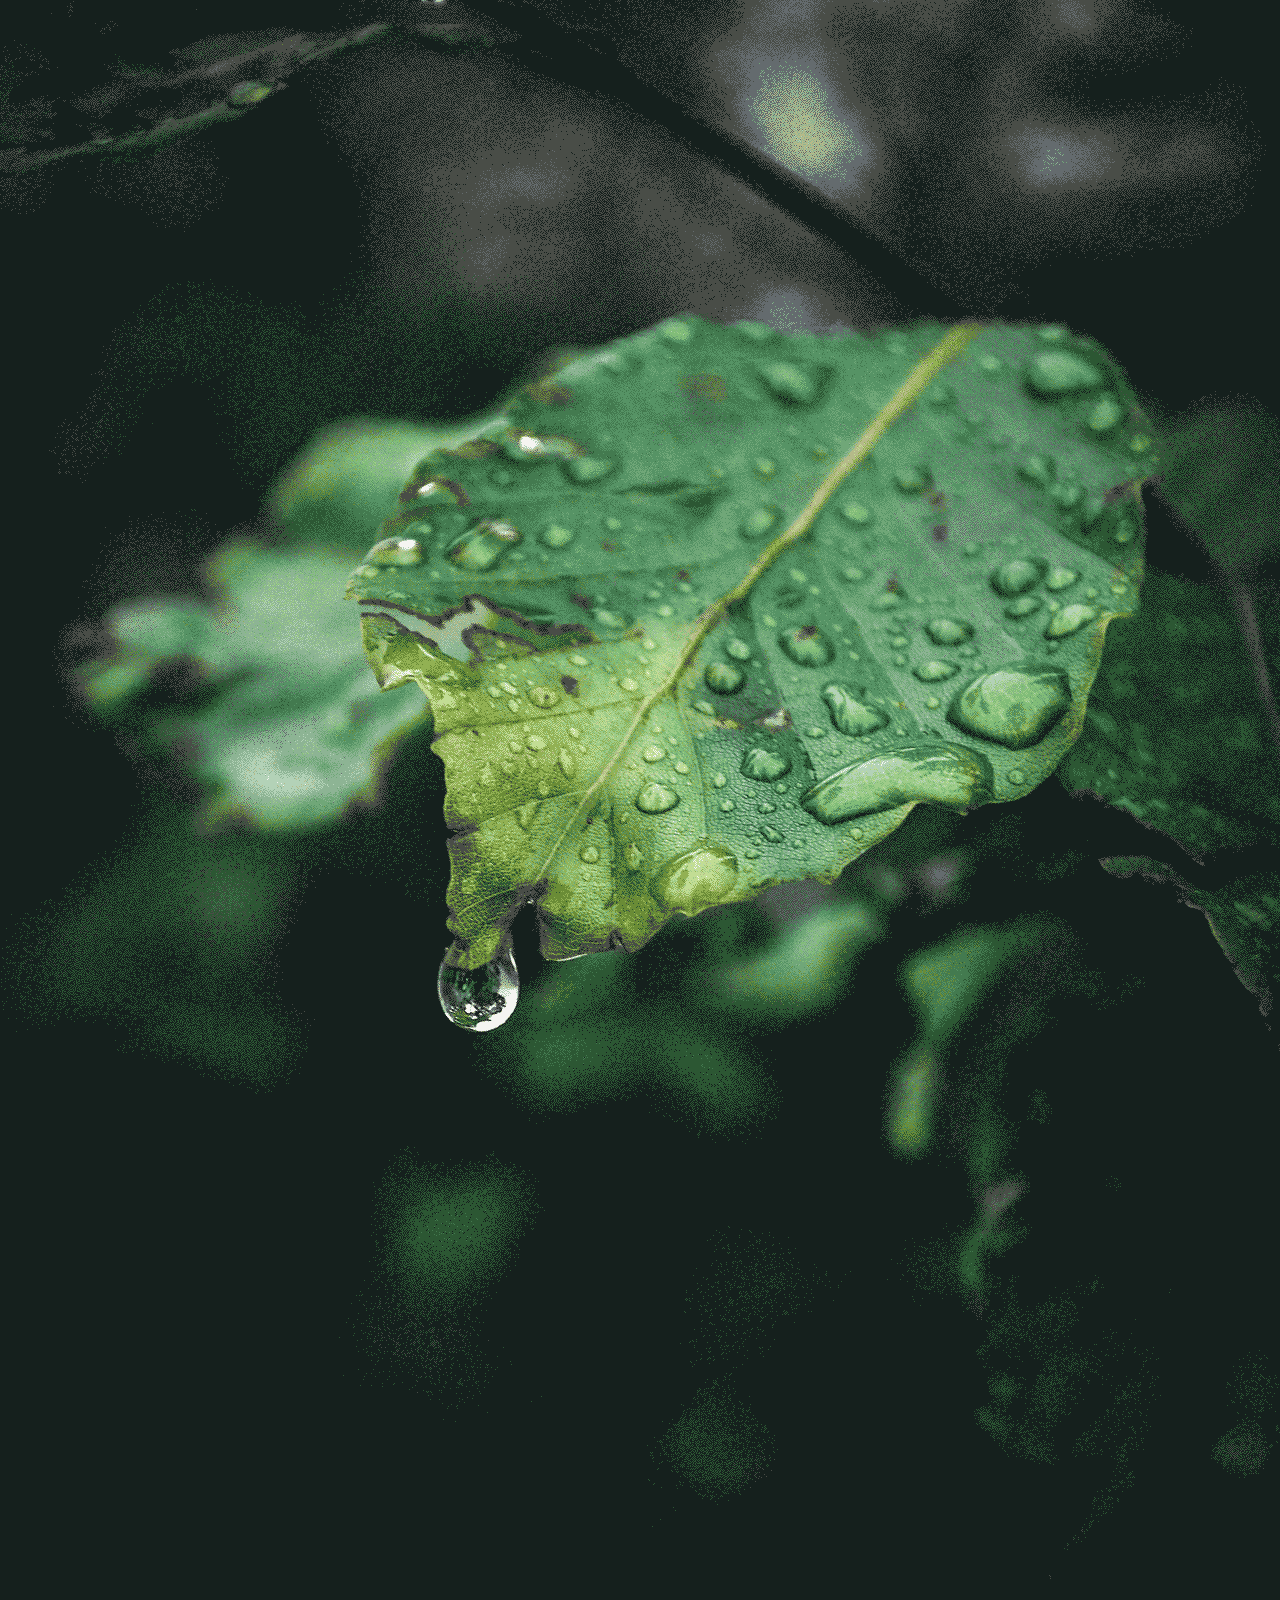
\includegraphics[width=\textwidth]{DMD/DitheringExamples/leaf16noise}
        \caption{16 colours, random dither}
    \end{subfigure}
    \caption[The effect of dithering on the perceived colour depth and quality of a downsampled image]{The effect of dithering on the perceived colour depth and quality of a downsampled image. The quantisation error is clearly visible in (b) but unless looked at from very close, (c) and (d) look very close to the original. Error diffusion and random dither achieve similar looking results, but the noise in case (d) is much more noticeable.\protect\footnotemark}
    \label{fig:dmd_dithering_example}
\end{figure}
\footnotetext{Software used: Adobe Photoshop (Version 21.0.0)}
%
For the decision which colour is assigned to each pixel during dithering, there are multiple algorithms available. One of the first developed is the Floyd-Steinberg algorithm (Alg.~\ref{alg:floyd_steinberg}, \cite{floydsteinberg:1976}) which is still highly used today. In this algorithm, the image is quantised from left to right and from top to bottom. The quantisation error of each pixel is diffused over the neighboring four pixels to the right and bottom. For the production of black and white image from grayscale values, an example of this is shown in Figure~\ref{fig:floyd_steinberg}
\begin{figure}[htbp]
    \centering
    \usetikzlibrary{arrows}
% \tikzset{marrow/.style={-latex,color={rgb:blue,1;green,6;white,2}}}
% \tikzset{marrow/.style={-latex,color=progression1!76!white}}
% \tikzset{mstyle/.style={rectangle,rounded corners,fill=black!80!white,opacity=0.75,draw=none}}
\tikzset{mstyle/.style={rectangle,rounded corners,fill=black!20!white,text=progression4,fill opacity=0.75,text opacity=1,draw=none}}

\tikzset{
  double -latex/.style args={#1 colored by #2 and #3}{    
    -latex,line width=#1,#2,
    postaction={draw,-latex,#3,line width=(#1)/3,shorten <=(#1)/4,shorten >=4.5*(#1)/3},
  }
}
\tikzset{marrow/.style={double -latex=1.5 pt colored by progression4 and white}}
\begin{tikzpicture}[scale=2]
    \begin{scope}
        \foreach \x in {0,1,2} {
            \shade[draw=none, inner color=black!65!white, outer color=gray!65!white] (\x,2) rectangle (\x + 1, 3) node [midway,color=white] {\huge $\checkmark$};
        }
        \shade[draw=none, inner color=black!65!white, outer color=gray!65!white] (0,1) rectangle (1, 2)  node [midway,color=white] {\huge $\checkmark$};
        \fill[draw=none, color={rgb:black,48;white,207}] (1,1) rectangle (2,2) node [midway,color=black] {207};
        \fill[draw=none, color={rgb:black,232;white,23}] (2,1) rectangle (3,2) node [midway,color=white] {23};
        \fill[draw=none, color={rgb:black,213;white,42}] (0,0) rectangle (1,1) node [midway,color=white] {42};
        \fill[draw=none, color={rgb:black,129;white,127}] (1,0) rectangle (2,1) node [midway,color=white] {127};
        \fill[draw=none, color={rgb:black,184;white,72}] (2,0) rectangle (3,1) node [midway,color=white] {72};
        \foreach \x in {0,1,2,3}{
            \draw (\x,0) -- (\x,3);
            \draw (0,\x) -- (3,\x);
        }
    \end{scope}

    \draw[-latex] (3.25,1.5) -- (4.25,1.5) node [midway,below=6pt] {$\Delta = -48$};

    \begin{scope}[xshift=4.5cm]
        \foreach \x in {0,1,2} {
            \shade[draw=none, inner color=black!65!white, outer color=gray!65!white] (\x,2) rectangle (\x + 1, 3)  node [midway,color=white] {\huge $\checkmark$};
        }
        \shade[draw=none, inner color=black!65!white, outer color=gray!65!white] (0,1) rectangle (1, 2)  node [midway,color=white] {\huge $\checkmark$};
        \fill[draw=none, color={rgb:black,0;white,255}] (1,1) rectangle (2,2) node [midway,color=black] (X) {255};
        \fill[draw=none, color={rgb:black,253;white,2}] (2,1) rectangle (3,2) node [midway,color=white] (R) {2};
        \fill[draw=none, color={rgb:black,225;white,35}] (0,0) rectangle (1,1) node [midway,color=white] (L) {35};
        \fill[draw=none, color={rgb:black,143;white,112}] (1,0) rectangle (2,1) node [midway,color=white] (B) {112};
        \fill[draw=none, color={rgb:black,186;white,69}] (2,0) rectangle (3,1) node [midway,color=white] (BR) {69};
        \foreach \x in {0,1,2,3}{
            \draw (\x,0) -- (\x,3);
            \draw (0,\x) -- (3,\x);
        }
        \draw[marrow] (X) .. controls (2,1.5) .. (R) node [midway,mstyle,above=2pt] {$\cdot 7/16$};
        \draw[marrow] (X) .. controls (0.75,1.25) .. (L) node [mstyle] at (0.6,1.1) {$\cdot 3/16$};
        \draw[marrow] (X) .. controls (1.5,1) .. (B) node [mstyle] at (1.5,1.1) {$\cdot 5/16$};
        \draw[marrow] (X) .. controls (2.25,1.25) .. (BR) node [mstyle] at (2.4,1.1) {$\cdot 1/16$};

    \end{scope}
\end{tikzpicture}
    \caption[Example for the application of the Floyd-Steinberg error diffusion algorithm]{Example for the application of the Floyd-Steinberg algorithm. When the central pixel is quantised to white (255), the error is diffused to the neighbouring pixels with the indicated ratios.}
    \label{fig:floyd_steinberg}
\end{figure}

Another possible dithering algorithm is to use random thresholds instead of fixed ones. For the production of binary patterns from grayscale images, this would mean to compare each pixel value against a random number between 0 and 1 instead of \num{0.5} for all pixels, which results in a very noisy image \cite{funkhouser:2000}. This method will therefore not be used here.

\section{Experimental Setup}
\label{sec:dmd_experimental_setup}
In the following section I will briefly describe the current experimental setup for the production of two-dimensional Bose gases which was already mentioned in the motivation for this part. The lower dimensionality is reached by \enquote{freezing} out one direction, meaning that the atoms do not have enough kinetic energy to populate the motional energy states in that direction. This is done with two sheet-beams coming from a DMD in the Fourier plane of the corresponding imaging lens. The interference of these beams creates a 1D lattice in the science cell. However, this only confines the atoms in one plane, where they could still move freely. For the additional in-plane confinement, another DMD is used to cut out a rectangle from a large-diameter blue-detuned beam which produces a dark centre trap (see Fig.~\ref{fig:bec2_trap_setup}).
\begin{figure}[htbp]
    \centering
    \begin{subfigure}[t]{0.48\textwidth}
        \centering
        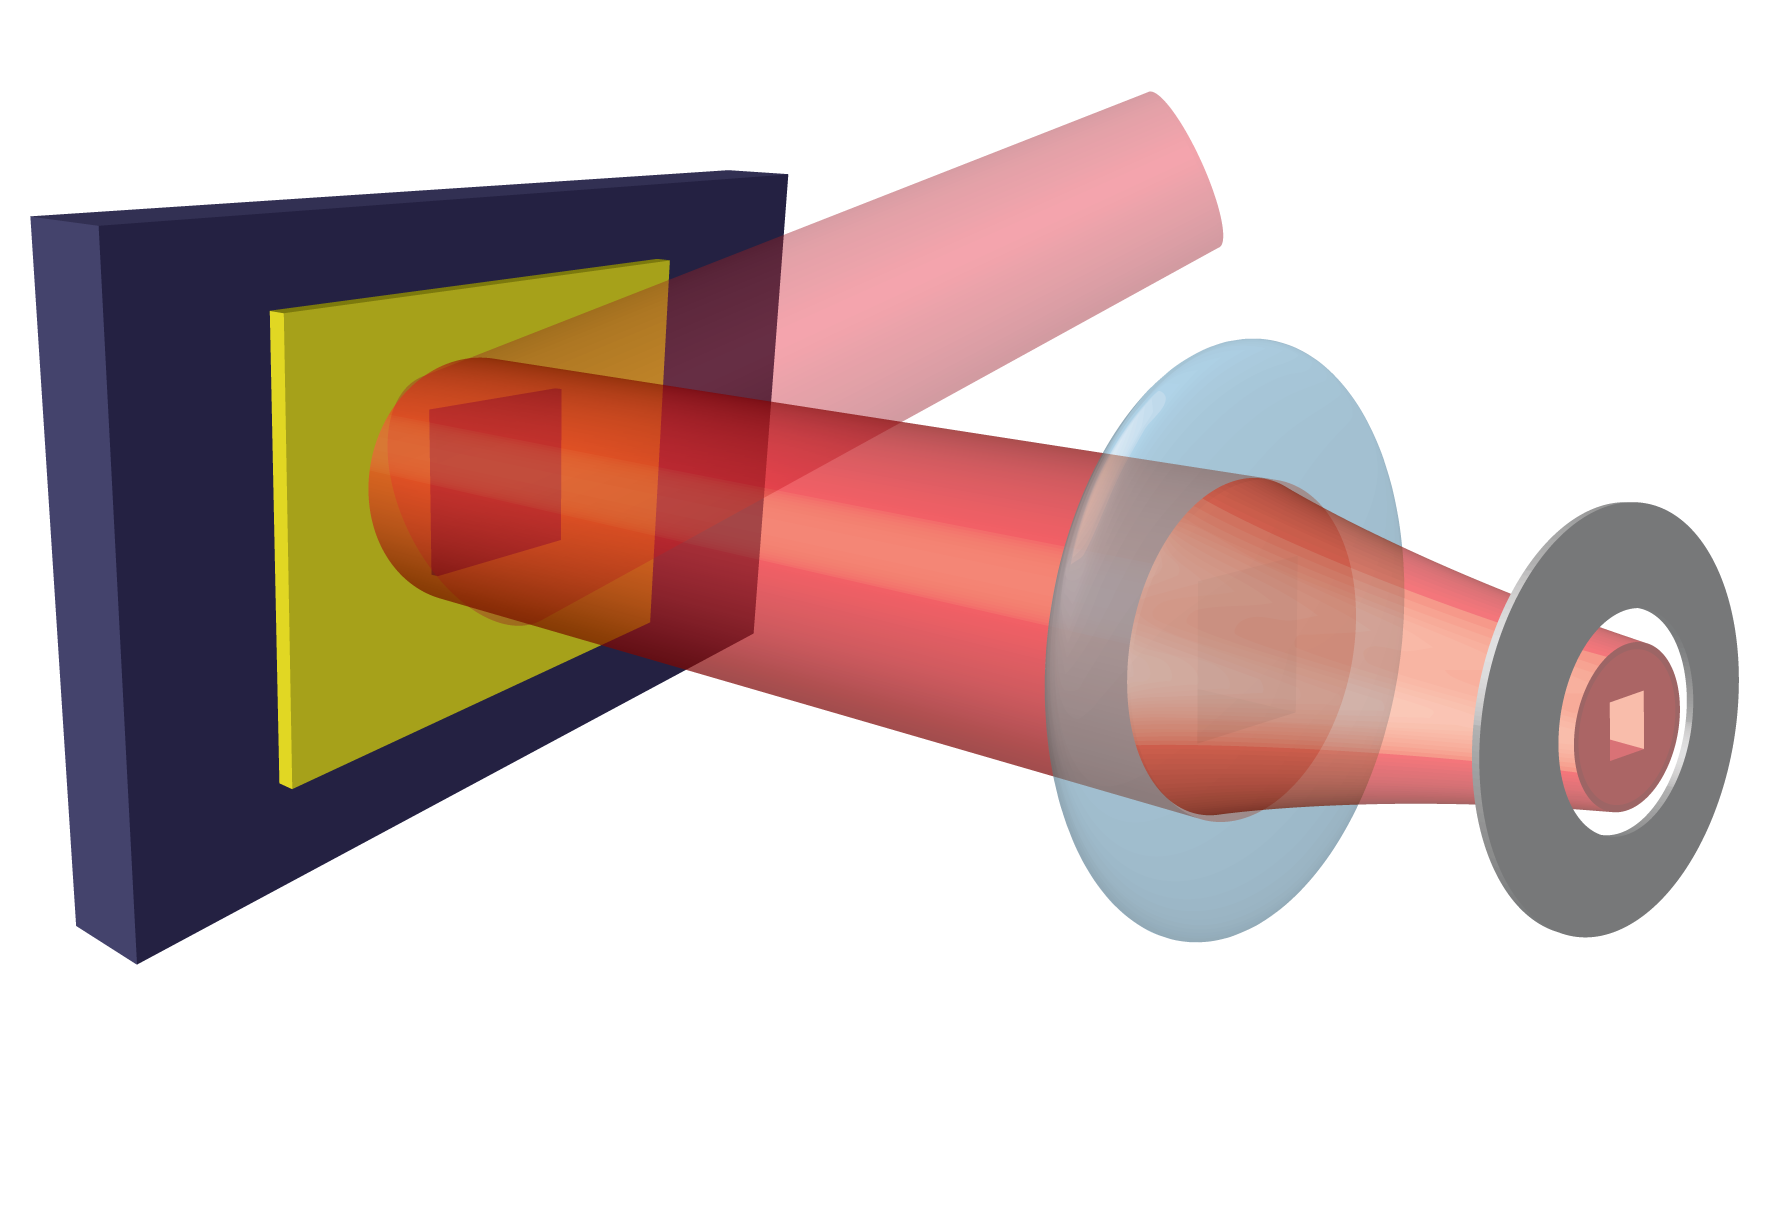
\includegraphics[width=\linewidth]{DMD/BEC2/box}
        \caption{Rectangular box (horizontal confinement)}
    \end{subfigure}
    \begin{subfigure}[t]{0.48\textwidth}
        \centering
        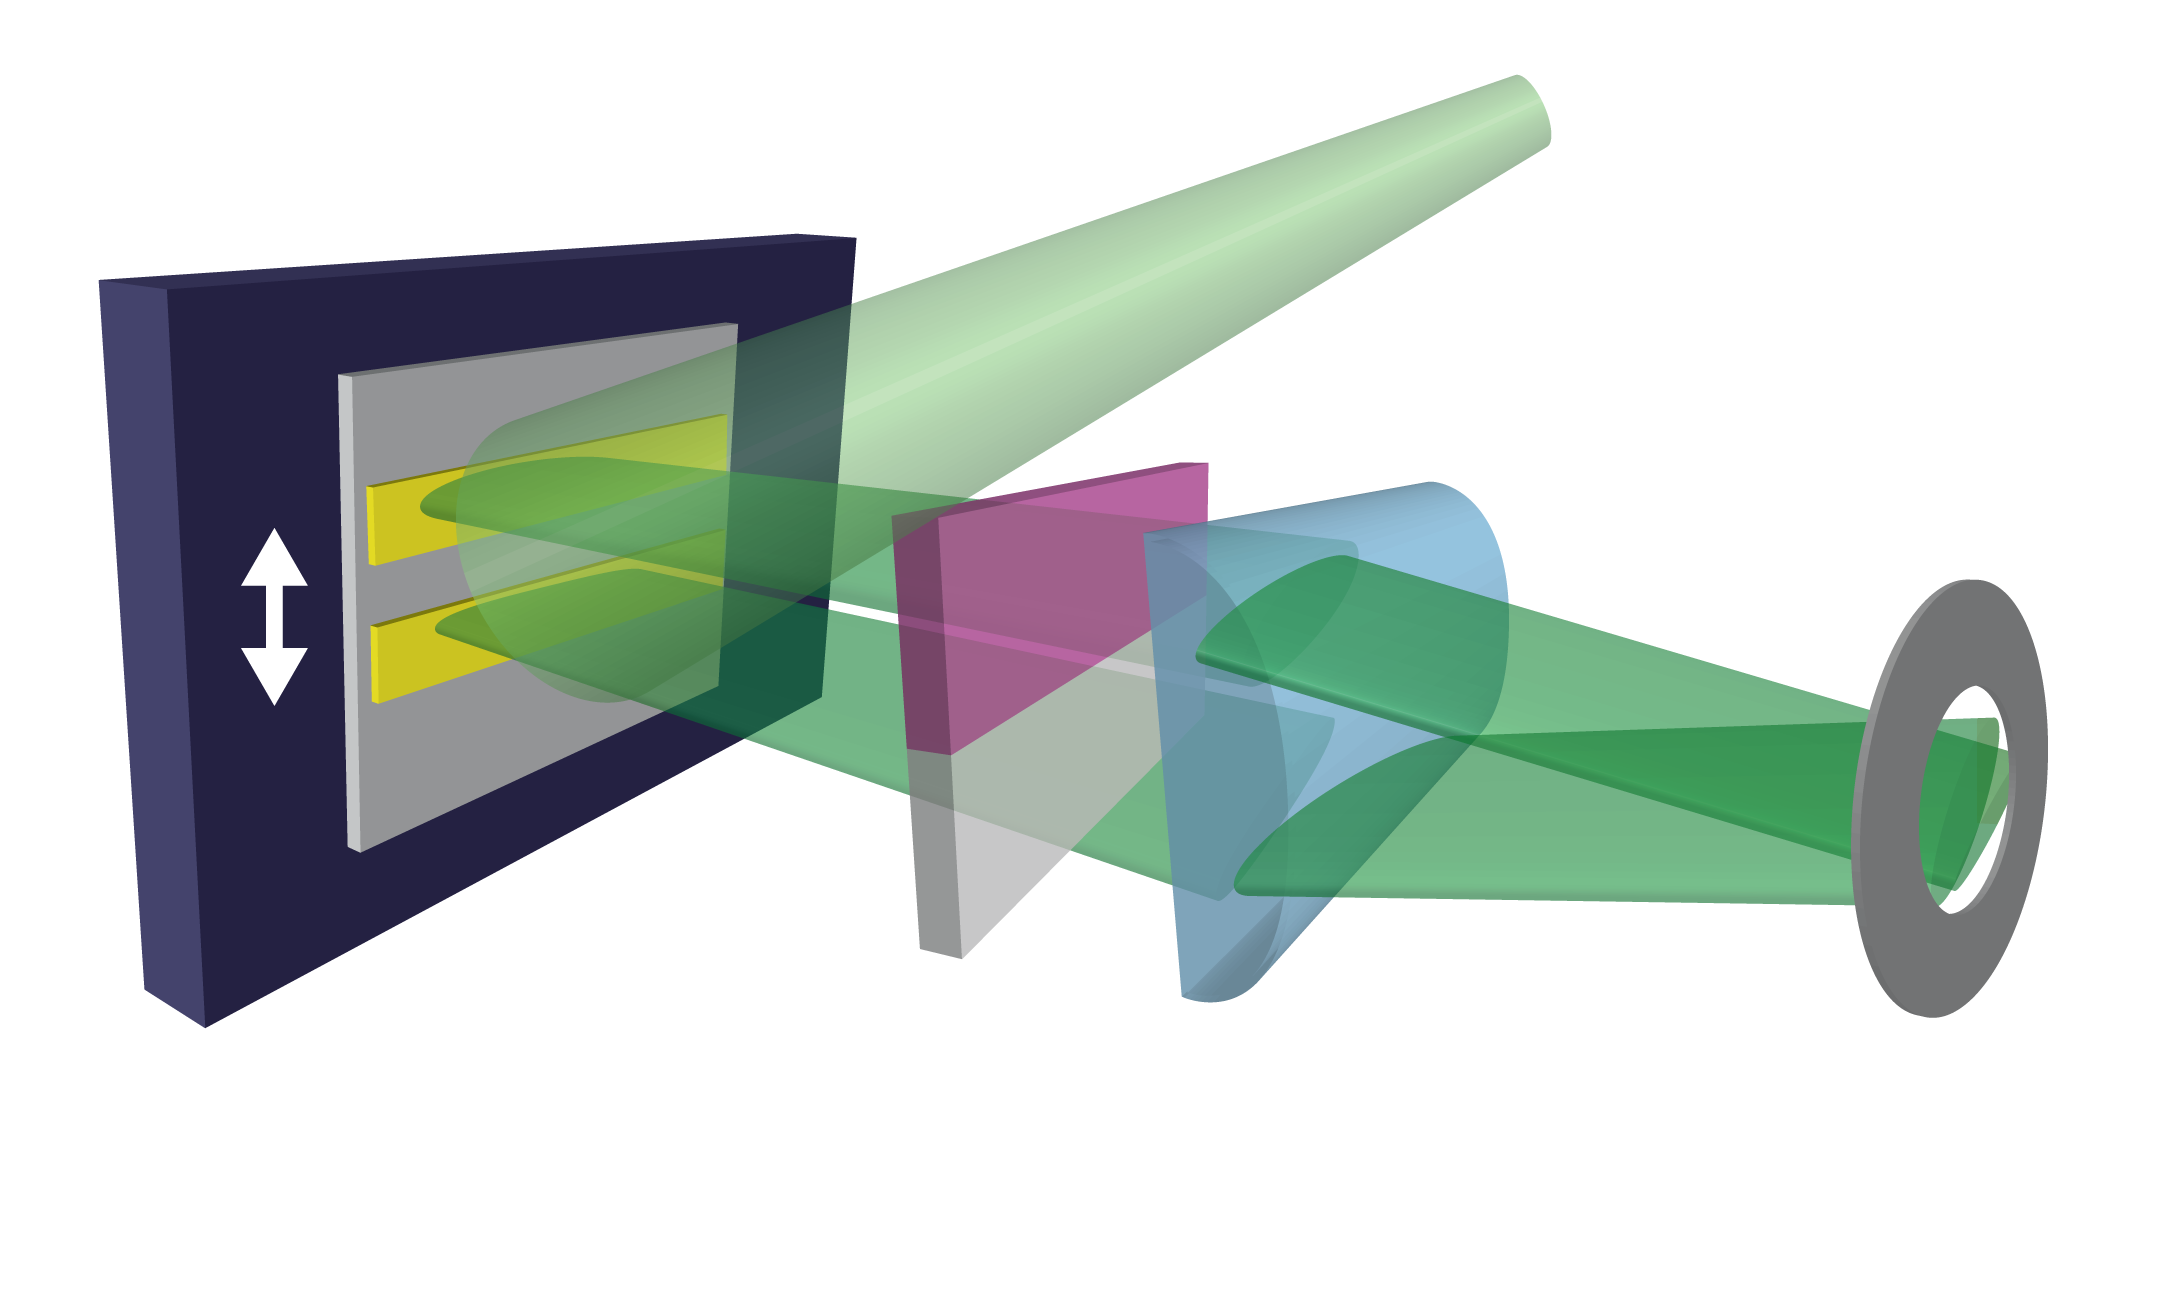
\includegraphics[width=\linewidth]{DMD/BEC2/sheets}
        \caption{Thin light sheets (vertical confinement)}
    \end{subfigure}
    \\ \vspace{1ex}
    \begin{subfigure}[t]{0.7\textwidth}
        \centering
        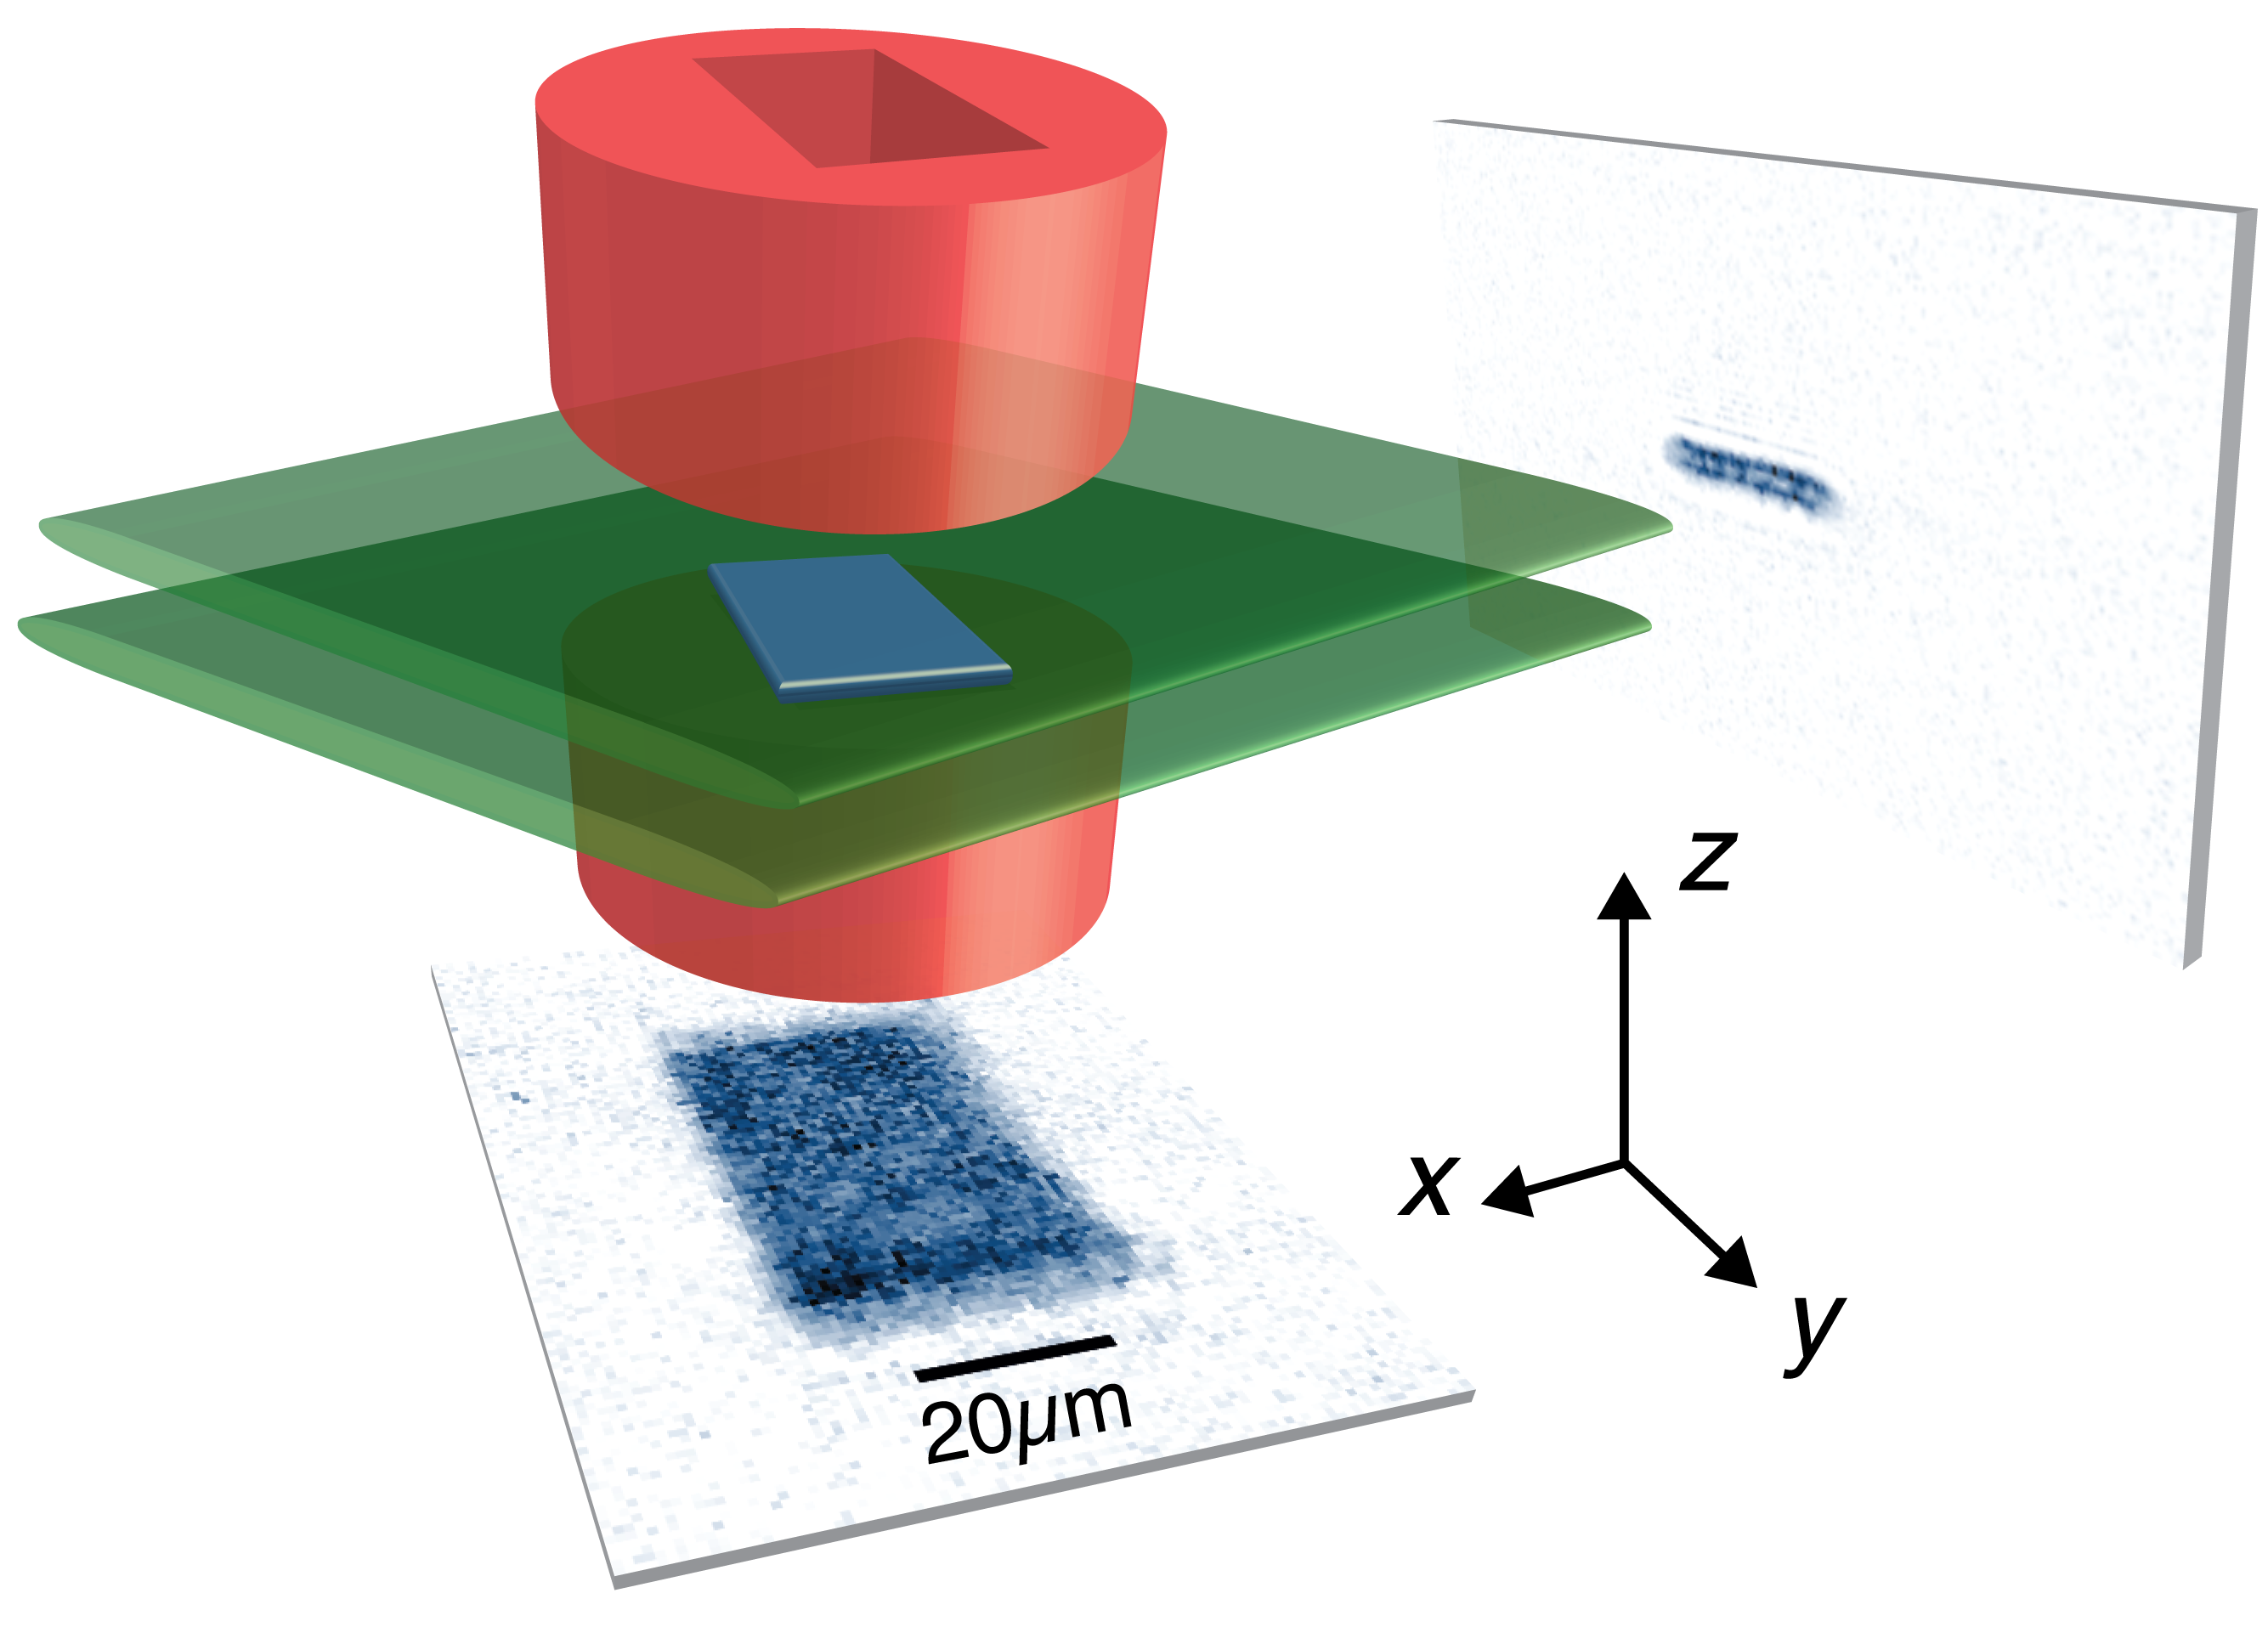
\includegraphics[width=\linewidth]{DMD/BEC2/complete}
        \caption{Full trap with atomic distribution}
    \end{subfigure}
    \caption[Optical box potential for two-dimensional Bose fluids]{Optical box potential for two-dimensional Bose fluids. Figures by J.~Schmitt, see also P.~Christodoulou et al.\ (in prep).}
    \label{fig:bec2_trap_setup}
\end{figure}
The problem that has been discovered and which motivated the development of a new correction algorithm is that there is some stray light in the supposedly dark centre of the trap with an intensity on the order of $<\!\SI{5}{\percent}$ of the intensity of the surrounding walls. This extraneous light, which most likely comes from the transverse trapping beams, disturbs the otherwise flat atomic distribution. One possibility for the origin of this effect are imperfections in the anti-reflective coating of the science cell which could lead to unwanted reflections of parts of the light used for the creation of the potential.

\section[Past Works]{Quick Review of Past Works}
In the past, two projects on DMDs have been done in our research group \cite{krstajic,bartlett}. Both of these worked on corrections for DMD patterns but focused mainly on the generation of flat top beams. To accomplish this, two different algorithms have been suggested for the optimisation of the imaged pattern. The first uses a feedback driven algorithm that takes the intensity error from a camera image and adds it to the projected pattern with a negative feedback constant with the goal to converge to the target pattern over several iterations.%:
% \begin{equation}
%     I_{n+1} = I_n + m\cdot \tanh (I_n - I_\text{target})
% \end{equation}
% The $\tanh$ function is used to suppress large fluctuations between iterations. Larger deviations are treated more gradually.

The second algorithm uses a mask produced from the intensity profile when the whole DMD is set to \emph{ON}. This mask can be applied to other images and assumes that imaging errors stay the same compared to the all-\emph{ON} case. In this second report, another method was mentioned where maxima and minima in the error intensity are reduced gradually by turning random pixels on or off in the respective region \cite{liang:2010}. However, this method was not further explored or implemented. 
The reported minimum RMS intensity deviations achieved for flat-top beams were \SI{4}{\percent} \cite{krstajic} and \SI{6}{\percent} \cite{bartlett} respectively.
Both reports emphasised that the calibration process, i.e.\ the process of mapping the camera pixels to the corresponding DMD pixels is critical for any kind of correction. This becomes especially true for patterns with high spatial variations.

% \vspace{1ex}\noindent
% Unfortunately, all the code that was written for these projects was in Matlab and the control software currently in use in the running experiment is written using \Cpp in the Qt framework. The algorithms developed in this work are all integrated into this control software. 